\chapter{GEMA}
Die \gls{gema} ist eine staatlich legitimierte Verwertungsgesellschaft, die durch ihre Arbeit das Ziel verfolgt, die Urheber von Musikstücken zu schützen. Sie vertritt damit die Interessen von Komponisten, Textdichtern und Verlegern. Das Konzept, welches hinter der \gls{gema} steckt, ist einfach. Überall dort, wo Musik gespielt wird, zum Beispiel in Einkaufszentren oder Konzerten, erhalten die Veranstalter durch die Musik einen finanziellen Vorteil. Dieser soll auch die Urheber der Musik, also die Komponisten, Textdichter usw. erreichen. Aus diesem Grund müssen Veranstalter, wenn sie rechtlich geschützte Musik spielen möchten, dies bei der \gls{gema} anmelden. Sie zahlen Lizenzgebühren, welche nach Abzug der Verwaltungskosten an die Urheber ausgeschüttet werden.
\newline
Im Folgenden soll näher auf die Entstehungsgeschichte der Verwertungsgesellschaft eingegangen werden.
\section{Entstehungsgeschichte}
\glqq Um die Wende vom 19. zum 20. Jahrhundert kam in Deutschland der Gedanke auf, musikalische Aufführungsrechte kollektiv zu verwerten.\grqq \seFootcite{}{S.6}{KBR:GEMAHK} Im Zuge dieser sogenannten \textit{Tantiemenbewegung}\footnote{Abgeleitet von Tantieme: Ergebnisorientierte Ausschüttung an Unternehmer aber auch Komponisten usw. durch die GEMA.} wurde die \gls{gdt} und die \gls{afma} am 14. Januar 1903 gegründet. Der Begriff der Verwertungsanstalt wurde ebenfalls damals geprägt. Er gilt als Kurzform für \textit{Anstalt für musikalisches Aufführungsrecht}.
\newline
\newline
Versuche, eine Verwertungsgesellschaft zu etablieren, sind auch bereits im 19. Jahrhundert vorgenommen worden. So wurde am 10. Mai 1898 die Leipziger Anstalt gegründet, welche allerdings bereits nach einem Jahr aufgrund massiven Widerstandes von Seiten der Veranstalter, aber auch der Komponisten, kapitulieren musste. Die Veranstalter waren der Überzeugung, dass die Gebühren für das Spielen von Musikstücken bereits im Kaufpreis der Noten enthalten sei. Die Komponisten kritisierten, dass die Verleger innerhalb der Anstalt mehr Mitbestimmungsrechte besaßen, als die komponierenden Mitglieder. Die Komponisten gründeten einen Berufsverband\footnote{Genossenschaft Deutscher Komponisten.} am 30. September 1998, um ihre Belange besser geltend zu machen.\seFootcite{Vgl.}{S.6-8}{KBR:GEMAHK}
\newline
\newline
Auch die \gls{gdt} und \gls{afma} wurden kritisiert, allerdings waren sie besser organisiert, als ihr Vorgänger -- die Leipziger Anstalt -- und konnten daher länger bestehen. Zu Beginn des 20. Jahrhunderts wurden weitere Verwertungsgesellschaften in Deutschland gegründet. Unter anderem die \gls{ammre}\footnote{Gründung: 4. November 1909.}, welche bei der Gründung der \glqq Alten GEMA\grqq~am 16. Dezember 1915 assistierte. Diese, damals noch \textit{Genossenschaft zur Verwertung musikalischer Aufführungsrechte} genannt, wurde von den aus der \gls{gdt}/\gls{afma} ausgeschiedenen Komponisten gegründet.
\newline
\newline
Die große Anzahl verschiedener Verwertungsgesellschaften brachte einige Nachteile mit sich. So mussten Nutzer häufig an verschiedene Organisationen Lizenzgebühren entrichten, um das Gesamtrepertoire an Musikstücken zu nutzen. Zudem führte die Konkurrenz der Verwertungsgesellschaften zu höheren Verwaltungskosten für die Berechtigten, da sie mehrere Verwaltungsapparate finanzieren mussten. Dies führte dazu, dass die verschiedenen Gesellschaften schon früh an einer Zusammenarbeit interessiert waren.
\newline
In einem ersten Zusammenschluss am 20. Februar 1916, also zwei Monate nach Gründung der Alten GEMA, schlossen sich diese und die \gls{akm} zusammen zum ersten \textit{Verband zum Schutze musikalischer Aufführungsrechte für Deutschland}. Die Alte GEMA und die AKM bildeten damit den ersten Musikschutzverband Deutschlands. 
\newline
Der zweite Musikschutzverband wurde am 22. Juli 1930 zwischen der \gls{gdt}, Alten GEMA und AKM gebildet.
Diese Zusammenschlüsse entsprachen keiner Fusion, sondern einem Zusammenschluss zu einer GbR, dass heißt, die Rechte blieben bei den einzelnen Verwertungsgesellschaften.\seFootcite{Vgl.}{S.14-17}{KBR:GEMAHK}
\newline
\newline
In der Anfangszeit der Verwertungsgesellschaften in Deutschland gab es noch kein einheitliches Wahrnehmungsrecht. \glqq Verwertungsgesellschaften bildeten sich als staatsferne Organisationen.\grqq\seFootcite{}{S.17}{KBR:GEMAHK} Sie unterlagen damit dem Privatrecht: Urheberrecht, Vertragsrecht, Gesellschaftsrecht und Deliktsrecht.
\newline
Erst am 4. Juli 1933 erließen die Nationalsozialisten mit dem sogenannten \textit{Gesetz über die Vermittlung von Musikaufführungsrechten} ein besonderes Wahrnehmungsrecht. Dieses Gesetz führte zur Verstaatlichung der Verwertungsgesellschaften unter der \textit{Staatlich genehmigten Gesellschaft zur Verwertung musikalischer Urheberrechte} (Stagma), welche von 1933 bis 1945 eine rechtliche Monopolstellung inne hatte.
\newline
Die Stagma durfte nach Kriegsende weiterbestehen und wurde 1947 in die heutige GEMA umbenannt. Sie besitzt seitdem eine faktisch monopolartige Stellung in Deutschland, da keine weiteren Verwertungsgesellschaften existieren, die die Rechte der Urheber wahrnehmen.\seFootcite{Vgl.}{S.19-24}{KBR:GEMAHK}
\section{GEMA heute}

\begin{figure}[H] 
\centering 

\includegraphics[scale=0.15]{se-wa-jpg/gema} 
\caption[GEMA Logo]{GEMA Logo} 
\label{gema_logo} 
\end{figure}

Die GEMA ist, wie im obigen Teil beschrieben, eine Verwertungsgesellschaft, dass heißt, sie nimmt die Urheberrechte ihrer Mitglieder (Komponisten, Textdichter und Musikverleger) wahr und stellt sie dem Nutzer für eine Lizenzzahlung zur Verfügung. Zur Zeit verwaltet die GEMA die Rechte von über 65.000 Mitgliedern sowie zwei Millionen Berechtigten weltweit. Sie schützt das geistige Eigentum ihrer Mitglieder, indem sie sie angemessen entlohnt. Die GEMA ist wie ein wirtschaftlicher Verein (§22 BGB) organisiert und wird vom deutschen Patent- und Markenamt beaufsichtigt sowie vom Bundeskartellamt.\seFootcite{Vgl.}{}{AA:GEMAPAGE}
\newline
\subsection{Mitgliederstruktur}
\label{mitlgiederstruktur}
Wichtigste Organe der GEMA sind die Mitgliederversammlung, der Aufsichtsrat und der Vorstand. Die Mitgliederversammlung findet einmal im Jahr in Berlin oder München statt. Die Mitglieder lassen sich in Berufsgruppen und Arten der Mitgliedschaft unterscheiden. Bei den Berufsgruppen kann man zwischen Komponisten, Textdichtern und Musikverlegern unterscheiden. Darüber hinaus gibt es drei verschiedene Arten von Mitgliedschaften:
\newpage

\begin{enumerate}
\item Angeschlossene Mitglieder
\item Außerordentliche Mitglieder
\item Ordentliche Mitglieder
\end{enumerate}

1. Angeschlossene Mitglieder:
\newline
Angeschlossenes Mitglied kann jeder Komponist, Textdichter und Verleger werden. Sie gelten zwar nicht als Mitglieder nach dem Vereinsrecht, bekommen allerdings trotzdem ihre Ausschüttungen ausgezahlt wie vollwertige Mitglieder. Wenn man den Aufnahmeprozess der GEMA durchlaufen hat, ist man automatisch ein angeschlossenes Mitglied. Diese Art der Mitgliedschaft ist Komponisten vorbehalten, die unregelmäßig musikalische Stücke veröffentlichen.
\newline
\newline
2. Außerordentliche Mitglieder:
\newline
Eine außerordentliche Mitgliedschaft muss beantragt werden. Hierfür sind bestimmte Voraussetzungen nötig. Unter anderem muss ein außerordentliches Mitglied mindestens fünf Notenmanuskripte beziehungsweise fünf veröffentlichte Tonträger vorweisen können.
\newline
\newline
3. Ordentliche Mitglieder:
\newline
Nach fünf Jahren als außerordentliches Mitglied kann eine ordentliche Mitgliedschaft beantragt werden. Neben diesen fünf Jahren müssen weitere Voraussetzungen erfüllt sein. Dabei spielt das erwirtschaftete GEMA-Aufkommen eine besondere Rolle. 
\newline 
\newline
Die Unterschiede der Mitgliedsarten liegen in der Stimmberechtigung für die Mitgliederversammlungen. Stimmberechtigt sind dabei nur ordentliche Mitglieder sowie 64 Delegierte der außerordentlichen und angeschlossenen Mitglieder.\seFootcite{Vgl.}{S. 1-3}{G:GEMAMF}
\newline
2015 lagen die offiziellen Mitgliederzahlen bei 56.143 angeschlossenen, 6.395 außerordentlichen und 3.825 ordentlichen Mitgliedern. Das macht insgesamt 66.363 Mitglieder in Deutschland.\seFootcite{Vgl.}{S.52}{GEMA:FB}

\subsection{Vergütung}
\glqq Verwertungsgesellschaften sind nach dem Urheberwahrnehmungsgesetz (UrhWahrnG) verpflichtet, Tarife über die Vergütung aufzustellen, die sie aufgrund der von ihr wahrgenommenen Rechte und Ansprüche fordert. Berechnungsgrundlage für die Tarife sind grundsätzlich die geldwerten Vorteile[...]\grqq\seFootcite{}{Abs. 4}{HR:GEMAWEB}, dass heißt, Musikstücke müssen nach einen klaren System tariflich eingeordnet und bewertet werden. Die GEMA hat dafür ein Punktesystem entwickelt, welches jedes Musikstück, ob Unterhaltungs-\footnote{Zum Beispiel Pop Musik.} oder \glqq Ernste\grqq-\footnote{Zum Beispiel klassische Musik.}Musik, bewertet und darauf aufbauend den Tarif für die Nutzung des Stücks festlegt. Bei der Einordnung wird nicht allein der Musiktyp berücksichtigt sondern auch die Dauer des Stücks. Entgegen der allgemeinen Meinung müssen auch schon für kleinste Teile eines Lieds Lizenzgebühren gezahlt werden.\seFootcite{Vgl.}{}{HR:GEMAWEB}
\newline
Wenn nun ein Veranstalter ein Konzert, Theater oder sonstiges plant, und dort durch die GEMA geschützte Musik spielen möchte kann er über deren Website (\texttt{https://www.gema.de/musiknutzer/musik-lizenzieren/}) sich und seine Veranstaltung anmelden. Aufbauend auf der Anmeldung wird dann die Lizenzgebühr berechnet. Die Höhe der Lizenzgebühren ist von verschiedenen Faktoren abhängig: Unter anderem der Musik, Teilnehmeranzahl, Veranstaltungsfläche und Dauer der Veranstaltung.
\newline
\newline
Der gesamte Prozess, von der Anmeldung bis zur Vergütung der Urheber, ist in \vref{gema_verguetung} dargestellt.

\begin{figure}[H] 
\centering 
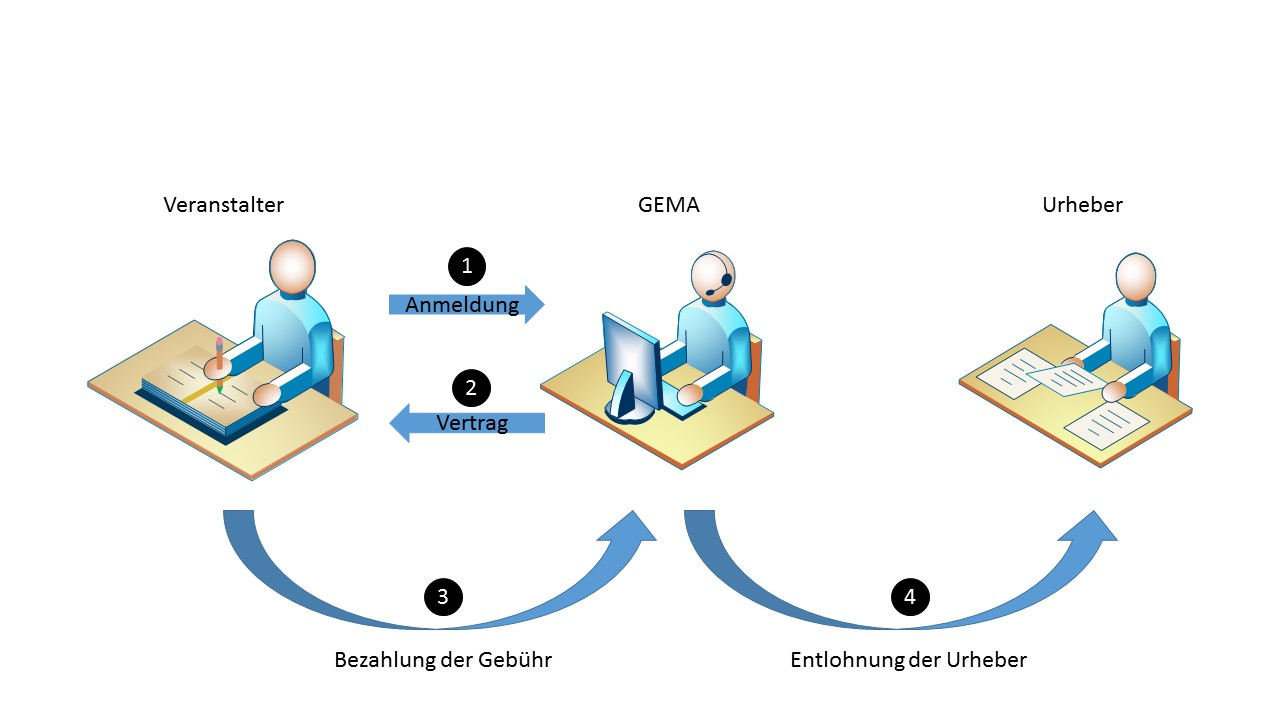
\includegraphics[scale=0.46]{se-wa-jpg/gema_verguetung} 
\caption[GEMA Vergütungssystem]{GEMA Vergütungssystem} 
\label{gema_verguetung} 
\end{figure}